\chapter{Multi-samples analyses with barcode sequencing}\label{ch:npbarcode}
\thispagestyle{empty}
\vspace*{\fill}
\epigraph{\emph{The more you read, the better you get at it.}}
{--James Patterson}

\clearpage
%%%%%%%%%%%%%%%%%%%%%%%%%%%%%%%%%%%%%%%%%%%%%%%%
The first part of this chapter presents a demultiplex algorithm that can be applied together with a barcode Nanopore sequencing in order to analyze multiple samples simultaneously in real-time. This practice is favorable for microbial genomics when the genome size is relatively small and a single flow cell can normally host more than one isolate for a run. As the result, a combination of barcode sequencing and streaming analysis can further reduce the overuse of resources.

The concept for such real-time demultiplexer has been implemented in \npbarcode{} and published in the \emph{Bioinformatics} journal article, namely \emph{"Real-time demultiplexing Nanopore barcoded sequencing data with \npbarcode{}"} as shown below. Its content will be adopted with additional details for the first section of this chapter. 
As the first author of this paper, I am the primary designer and software developer of the project. I contributed significantly to data generation, interpretation as well as writing the first draft of the manuscript.

Later in this chapter, an use case will be addressed as a highlighted example of genome assembly practices to resolve an actual problem in research. \npscarf{} with other state-of-the-art assembly methods are employed for such task.
The data being presented in this section is part of another study, namely \emph{"Evaluating the Genome and Resistome of Extensively Drug-Resistant Klebsiella pneumoniae using Native DNA and RNA Nanopore Sequencing"} which has myself as a co-author. 
In general, my contributions fall mostly in the bioinformatics aspects of the research.
I played a critical role in data processing and genome assembly, as well as partly in plotting and interpreting the final results.

The full manuscript with supplementary materials can be accessed via the preprint version from the link \url{https://doi.org/10.1101/482661}. The study has been submitted to \emph{Nature Microbiology} journal and is currently under review.

\clearpage
%%%%%%%%%%%%%%%%%%%%%%%%%%%%%%%%%%%%%%%%%%%%%%%%
%%%%%%%%%%%%%%%%%%%% Paper %%%%%%%%%%%%%%%%%%%%%
%\pagebreak
\thispagestyle{empty}
\vskip36pt
{\raggedright\sffamily\bfseries\fontsize{20}{25}\selectfont {Real-time demultiplexing Nanopore barcoded sequencing data with npBarcode}\par}
\vskip20pt
{\raggedright\sffamily\fontsize{12}{12}\usefont{OT1}{phv}{m}{n} {
\textbf{Son Hoang Nguyen}\textsuperscript{1,$\ast$},
\textbf{Tania Duarte}\textsuperscript{1},
\textbf{Lachlan J.M. Coin}\textsuperscript{1} and
\textbf{Minh Duc Cao}\textsuperscript{1,$\ast$}
}\par}
\vskip10pt
{\raggedright\sffamily\fontsize{10}{12}\usefont{OT1}{phv}{m}{n} {
\textsuperscript{1}Institute for Molecular Bioscience, University of Queensland, 
St Lucia, Brisbane, QLD 4072 Australia \par
\textsuperscript{$\ast$}Correspondence:
\href{s.nguyen@uq.edu.au}{s.nguyen@uq.edu.au} and 
\href{m.cao1@uq.edu.au}{m.cao1@uq.edu.au}.
}\par}
\vskip10pt
%%%%
{\raggedright\sffamily\fontsize{12}{16}\selectfont  {Received 20 Jun 2017. Accepted 23 Aug 2017. Published 24 Aug 2017}\par}
\vskip10pt
{\raggedright\sffamily\fontsize{12}{16}\selectfont  
PMID: 28961965 \hskip15pt DOI:~\href{https://doi.org/10.1093/bioinformatics/btx537}{10.1093/bioinformatics/btx537}\par}
\vskip10pt
\paragraph{Abstract}\mbox{}\\
\textbf{Motivation:} The recently introduced barcoding protocol 
to Oxford Nanopore sequencing has increased the versatility of the technology.
Several bioinformatics tools have been developed to demultiplex the barcoded 
reads, but none of them support the streaming analysis. This limits the use
of pooled sequencing in real-time applications, which is one of the main 
advantages of the technology.\\
\textbf{Results:} We introduced \npbarcode{}, an open source and cross platform 
tool for barcode demultiplex in streaming fashion. npBarcode can be seamlessly 
integrated into a streaming analysis pipeline. The tool also provides a friendly
graphical user interface through \npreader{}, allowing the real-time visual 
monitoring of the sequencing progress of barcoded samples. 
We show that
\npbarcode{} achieves comparable accuracy to the other alternatives. \\
\textbf{Availability:} \npbarcode{} is bundled in Japsa - a Java tools kit for 
genome analysis, and is freely available at 
\href{https://github.com/hsnguyen/npBarcode}{https://github.com/hsnguyen/npBarcode}.
\clearpage
\pagebreak

\section{Demultiplex barcode sequencing with MinION}
\subsection{Introduction}

Introduced only in 2014, Oxford Nanopore Technologies (ONT) sequencing has already become an established technology for its portability and its potential for high yield data generation. 
In particular, it offers the ability of real-time sequencing where practitioners can analyze data streaming directly from the sequencing device, and can terminate a sequencing run once the satisfactory results are obtained. Recently, ONT introduced barcode protocols to allow pooling and sequencing multiple libraries on the sample flow cell, which further enhances the versatility of the technology. The underlying mechanism is to ligate a unique oligonucleotide sequence, or \emph{barcode}, to the fragments of each DNA sample. Multiple samples can then be pooled together and sequenced in one flow cell. The sequenced reads can then be demultiplexed into bins by examining the barcode portions on the reads.

Several outstanding tools for demultiplexing Nanopore barcoded sequences such as poreFUME~\cite{Van2017rapid}, Porechop~\url{https://github.com/rrwick/Porechop} and Metrichor built-in demultiplexer have been developed. Of these tools, only the latter supports real-time analysis of a sequencing run, but it is only available as a cloud service. This limits the use of this technology in time-critical applications or when the users wish to perform sequencing only until sufficient data are obtained.

Being able to exploit the streaming property of nanopore sequencing is important for time-critical applications, especially when its data generating yield and rate is escalating drastically with new technologies and platforms already or soon become available such as GridION, PromethION.
Hence, algorithms that can work with streaming data and be able to integrated into a pipeline should be taken into consideration in earnest for this sequencing technology. Furthermore, a more friendlier user interface to inexperienced users is highly on demand as many more researchers worldwide are enrolled in MinION  multi-samples sequencing. In addition, the visualization can provide more efficient statistical report in real-time allowing users to have better control over the whole sequencing process.
For that reason, we developed another tool for ONT barcode sequencing demultiplex analysis. 

Here, we present \npbarcode{}, a sensitive tool for demultiplexing barcoded MinION sequencing data in real-time. \npbarcode{} provides the traditional command line interface and a graphical user interface.
The command line interface offers a flexible environment to be integrated in with other real-time downstream analyses, \emph{e.g.} real-time finishing genome sequence (\npscarf{}~\cite{Cao2017scaffolding}) and real-time 
species identification (npAnalysis\cite{CaoGE2016}). The demultiplexer is also integrated into \npreader{}'s~\cite{CaoGC2016}, our previously developed platform for real-time analysis and visualization of nanopore sequencing.
From this mode, beside the utilities provided by \npreader{}, one can visually monitor on the sequencing progress of each barcoded sample.

\subsection{Results}
\subsubsection{Algorithm overview}
\npbarcode{} relies on local pairwise alignment to detect the existence of a barcode sequence in each nanopore read. We apply the Smith-Waterman algorithm with Gotoh's optimization~\cite{Gotoh1982improved} for the alignment. Basically, 
the aligner attempts to align the barcode sequences within a window on both ends of a nanopore read. The read is assigned to the group of the barcode with the highest alignment score, provided that the score is greater than a threshold, and is greater than the second best alignment score by a safety distance.

\npbarcode{} is implemented within the Japsa toolkit as a program named $\mathtt{jsa.np.barcode}$.
The program consumes the base-called data in a streaming fashion and demultiplexes the data into different channels containing reads that belong to the same bin. 
These output streams can be piped to other downstream real-time analyses.
This design allows practitioners to integrate the tool into a streaming analysis pipeline of interests.

\subsubsection{Comparison with other methods}

\begin{figure}[ht]
\centerline{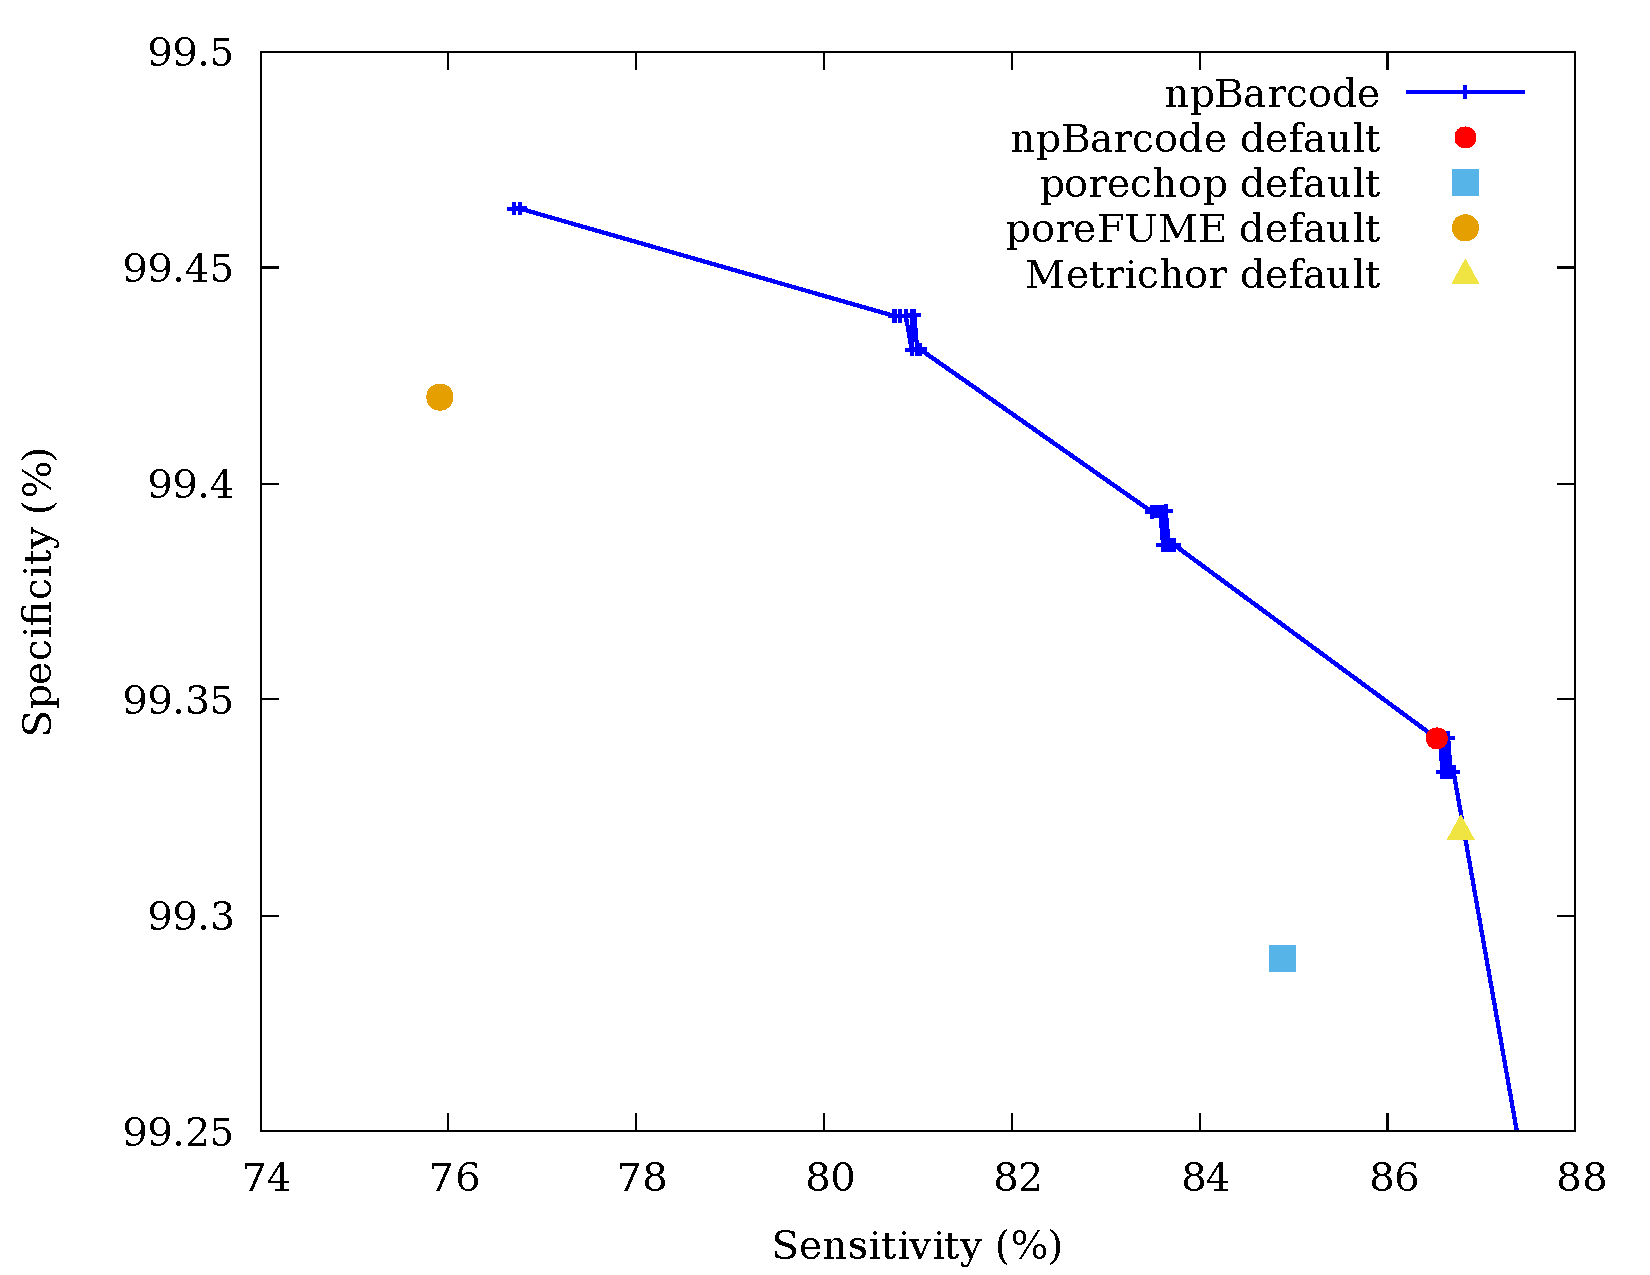
\includegraphics[width=0.6\textwidth]{images/roc.pdf}}
\caption{Plot of sensitivity versus specificity of \npbarcode{} compared
with existing tools.}
\label{fig:sen}
\end{figure}

We barcoded and sequenced 8 different bacterial strains on a single MinION R9.4 flow cell using the Oxford Nanopore Technology's 2D native barcoding kit (SQK-LSK208 + EXP-NDB002). Another run with PCR barcoding kit for 3 libraries is not discussed here as part of a different study, but its result is included in Appendix Figure~\ref{supp_fig:npbarcode_pcr}.

The pool consisted of one gram-positive isolate (\emph{Staphylococcus aureus}) and seven gram-negative isolates (four \emph{Klebsiella pneumoniae}, one \emph{Klebsiella quasipneumoniae}, one \emph{Pseudomonas aeruginosa} and one \emph{Acinetobacter baumannii}).
In order to establish a ground truth benchmark for  comparison of different de-multiplexing tools,  we aligned the sequence reads of the eight samples to their respective assemblies to identify the original source of the reads. 
Due to the high level of similarity among the gram negative isolates, we could only obtain the confident assignment of reads to the \emph{S. aureus}, a gram positive strain, versus the other gram negative strains. 
Hence, we set up the comparison framework as the accuracy of the tool detecting the barcode associated with the \emph{S. aureus} sample. For an exhaustive benchmark for each of every strains included, ones can assess Appendix Figure~\ref{supp_fig:comparison}.

Figure~\ref{fig:sen} presents the sensitivity and specificity of \npbarcode{} with differing parameters. We also obtained the results from Metrichor, porechop and poreFume with their default parameter settings. 
Statistics of all tools with their automatic settings is depicted in details in Appendix Table~\ref{supp_tab:sensitivity}.
We found that \npbarcode{} performed comparably with Metrichor and was marginally more accurate than the competitive porechop and poreFUME.


\subsubsection{Multiple samples real-time scaffolding pipeline}

\begin{figure}[!hpb]
\centering
\subfloat[\emph{K. pneumoniae} isolate 1]{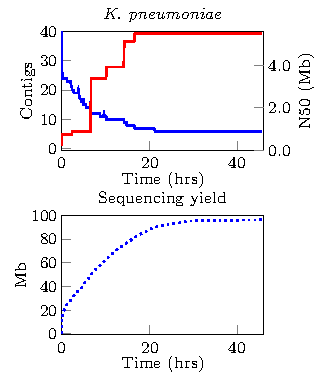
\includegraphics[width=0.30\textwidth]{images/s092.pdf}}%
\subfloat[\emph{K. pneumoniae} isolate 2]{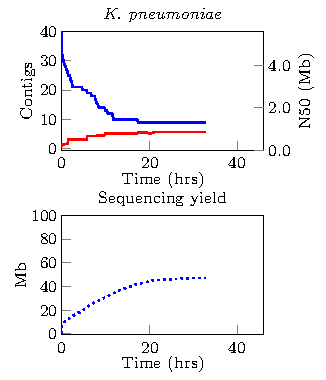
\includegraphics[width=0.30\textwidth]{images/s133.pdf}}%
\subfloat[\emph{K. pneumoniae} isolate 3]{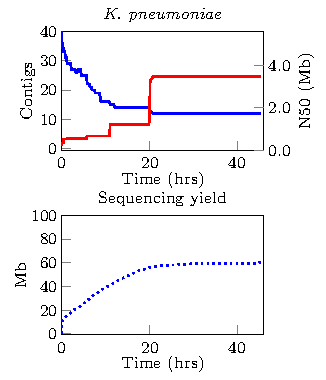
\includegraphics[width=0.30\textwidth]{images/s096.pdf}}%
\\
\subfloat[\emph{K. pneumoniae} isolate 4]{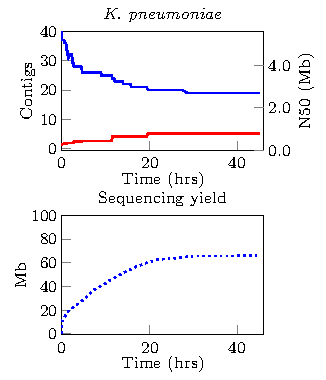
\includegraphics[width=0.30\textwidth]{images/s106.pdf}}%
%\hfill
\subfloat[\emph{K. quasipneumoniae} isolate]{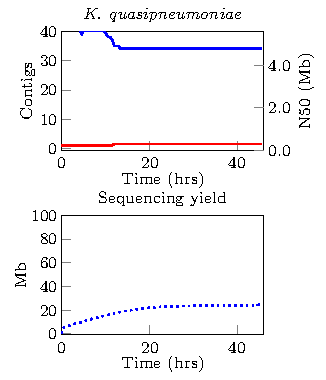
\includegraphics[width=0.30\textwidth]{images/s132.pdf}}%
%\hfill
\subfloat[\emph{A. baumannii} isolate]{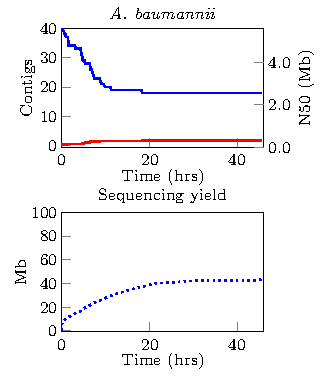
\includegraphics[width=0.30\textwidth]{images/s093.pdf}}%
%\hfill
\\
\subfloat[\emph{K. aeruginosa} isolate]{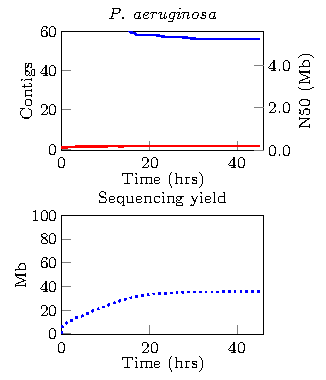
\includegraphics[width=0.30\textwidth]{images/s101.pdf}}%
%\hfill
\caption[A combining pipeline of \npreader{}, \npbarcode{} and \npscarf{} with ONT Native Barcoding Kit]{Result for running a combining pipeline of \npreader{}, \npbarcode{} and \npscarf{} with ONT Native Barcoding Kit in order to scaffold genomes of 7 gram-negative samples in real-time. For each sample, the upper plot shows number of contigs (blue) and N50 (red) while the lower graph presents data yield (bases) for that particular demultiplexed sample over time.}
\label{fig:scaffold}
\end{figure}

As part of the experiment, we also integrated \npbarcode{} into a streaming analysis
pipeline where we scaffolded genome assemblies in real-time. Prior 
to the MinION sequencing run, we sequenced the seven gram negative samples with
Illumina technology and used \spades{}~\cite{BankevichNA2012} to assemble them into
assemblies, which each had exceeding 
100 contigs. The \emph{S. aureus} sample was used as a control sample during 
demultiplexing, and was not used for scaffolding.
As soon as a sequence read was generated, it was base-called, demultiplexed and
streamed into the appropriate instance of \npscarf{}~\cite{Cao2017scaffolding} 
for scaffolding. This
pipeline allowed us to simultaneously scaffold all seven bacterial samples while
the sequencing was still in progress (Figure~\ref{fig:scaffold}). We were able 
to complete the genome of one \kp{} isolate after 16 hours of
sequencing and with about 80Mb of nanopore sequencing data. While the genomes of 
the other six isolates were not completed due to their low proportions in the 
pooled sample, and the less than ideal yield of the run, they were significantly
improved over time with nanopore long reads.

\subsubsection{Graphical user interface}

\begin{figure}[ht]
\centerline{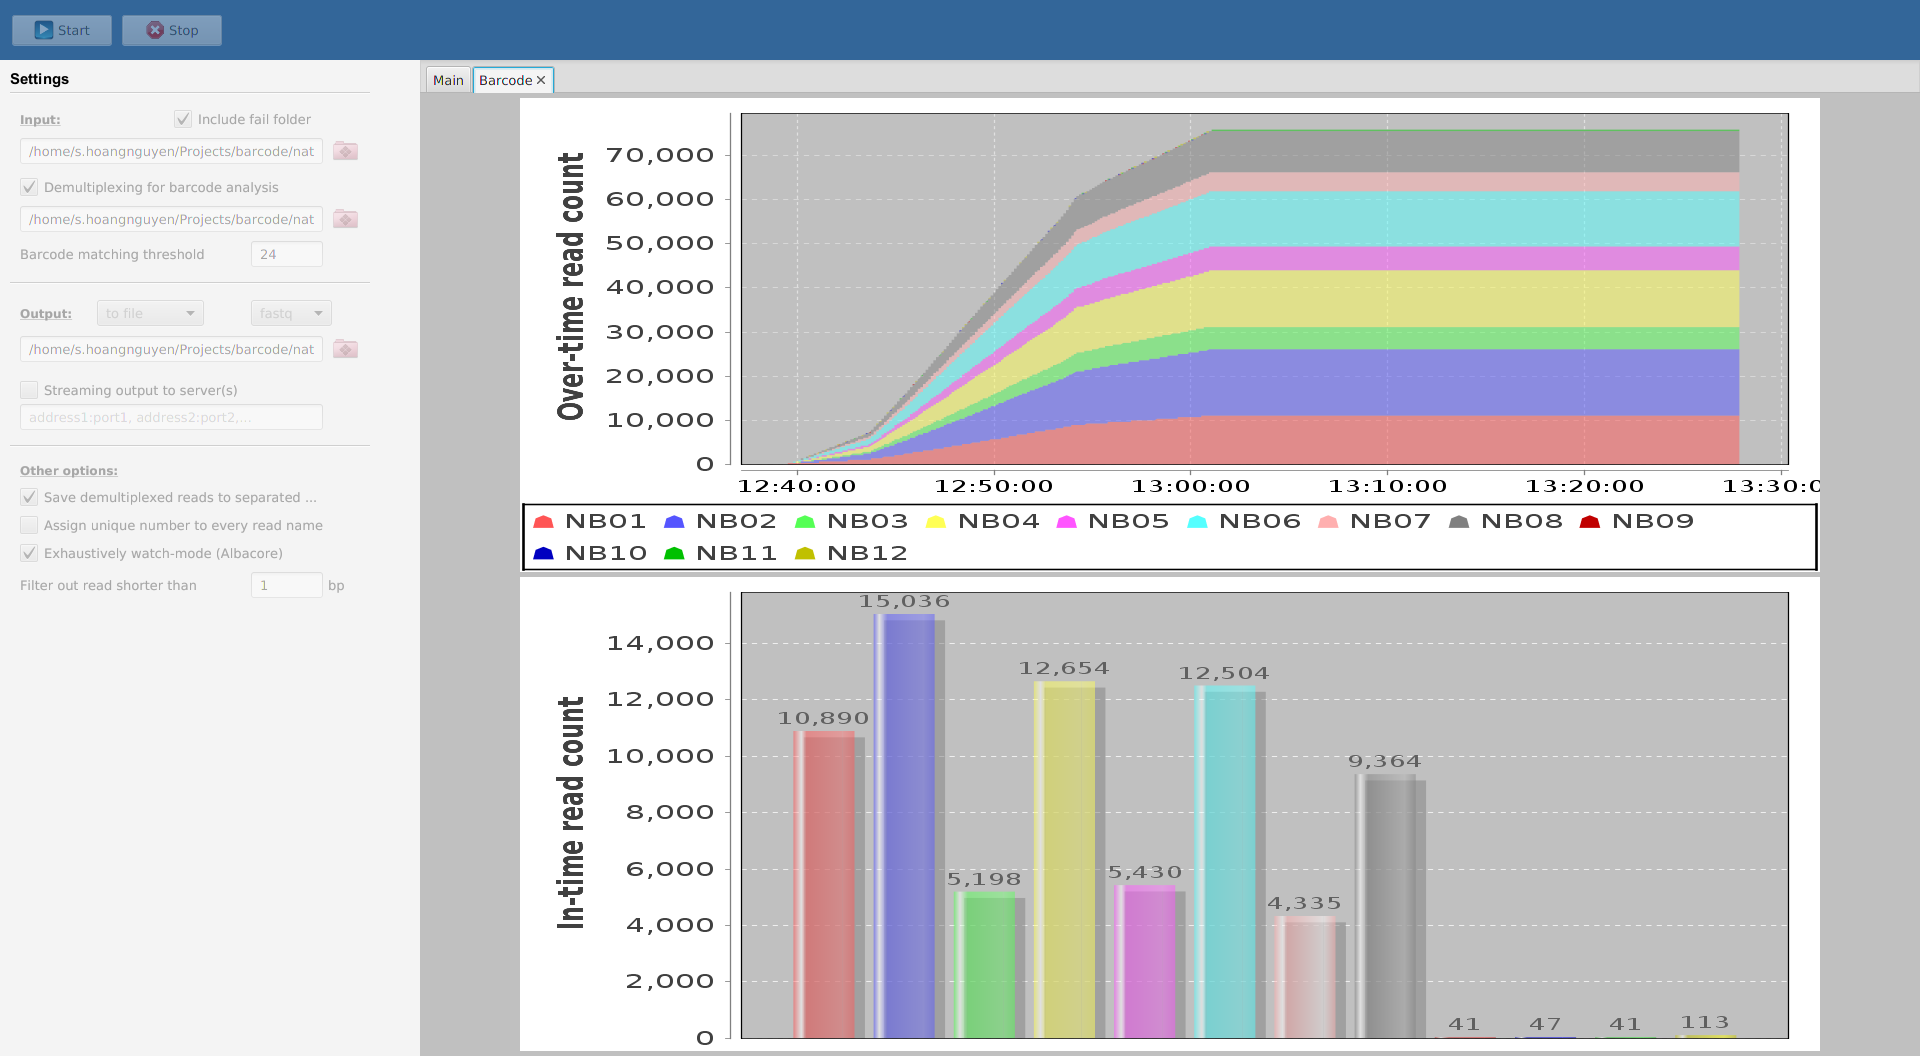
\includegraphics[width=0.9\textwidth]{images/native2.png}}
\caption{Graphical User Interface of npBarcode integrated in npReader. The 
result shown is for the a MinION run using Native barcoding kit on 8 libraries.}
\label{fig:gui_npbarcode}
\end{figure}
\npbarcode{} is also integrated into \npreader{}'s graphical user interface. With 
this, users can monitor the amount of sequencing data for each pooled sample
in real-time. When required, \npreader{} provides a view showing read-count per bin 
in a real-time fashion. This view provides two plots that can depict the progress 
in an over-time and in-time manner, respectively. The first scenario would offer 
more general progress viewing by showing the read count of the whole process 
while the lower graph figures the exact number of binned reads at a particular 
time point. An example of the visualization is shown in Figure~\ref{fig:gui_npbarcode}. 
Overall it reflects the 
demultiplex functioning appropriately with the majority of reads falling in the 
bins corresponding to the samples used for the barcode sequencing. Only an 
negligible  amount of reads are mis-classified into unrelated bins.

\subsection{Methods}
\subsubsection{Bacterial cultures and DNA extraction}
Bacterial strains include \emph{Streptococcus pneumoniae} sourced from the American Type Culture Collection (ATCC 700677) and various clinical isolates from Hygeia General Hospital, Athens, Greece or Instituto Dante Pazzanese de Cardiologia, Brazil~\cite{Miranda2018}. Clinical isolates comprise of four \emph{Klebsiella pneumoniae} (3\_GR\_13, 5\_GR\_13, 11\_BR\_13, 22\_GR\_12), \emph{Klebsiella quasipneumoniae} (21\_GR\_13), \emph{Acinetobacter baumannii} (source: Hygeia General Hospital, 2013) and \emph{Pseudomonas aeruginosa} (source: Hygeia General Hospital, 2013). It is worth noting that the sample identifiers are re-assigned for convenient as shown in Table~\ref{supp_tab:sample} which emphasize on the gram stain of the bacteria: GP for gram positive and GN for gram negative.
Bacterial cultures were supplied as stabs/slants or on agar, grown in nutrient broth or brain heart infusion broth, glycerol stocks were made to $20 \%$ (v/v) glycerol and stored at $−80^o$C.

For DNA extractions, glycerol stocks were struck out on either nutrient agar or tryptic soy agar with $5\%$ defibrinated sheep blood to isolate single colonies. Strains were grown overnight at $37^o$ shaking at 220 rpm and DNA subsequently extracted from this inoculum. DNA was isolated using the DNeasy Blood and Tissue Kit (Qiagen) with the additional enzymatic lysis buffer pre-treatment as per the manufacturer’s instructions. DNA was quantified with Qubit3.0 (ThermoFisher Scientific).
\subsubsection{Illumina sequencing and assembly}
One nanogram of DNA was used for the Nextera XT (Illumina) library preparation as per the manufacturer’s instructions and quality was evaluated via a 2100 Bioanalyzer (Agilent Technologies). Libraries were sequenced on an Illumina MiSeq (300 bp paired-end reads) with $>$100X coverage per sample.

The raw reads from each data set were processed by  $\mathtt{Trimmomatic}$~\cite{BolgerLU2014} version 0.36 to remove adapter sequences and attain paired reads only. After that, \spades{} 3.10.1 was used to generate short-read assembly consisting of high quality contigs.
\subsubsection{MinION barcode sequencing}
The same DNA extract from the Illumina sequencing run was used for Nanopore sequencing. The library preparation was done following the 2D native barcoding kit (SQK-LSK208 + EXP-NDB002) with the input between 900 to 1500 nanograms of DNA for each sample as in Table~\ref{supp_tab:sample}. 
The samples were pooled in equimolar concentrations and 15.75ng was loaded into a R9.4 FLOMIN106 flow cell. After 20 hours the flow cell was topped up with 6$\mu$L of library.

The sequencing run was stopped after 43 hours and generated 65,029 reads and 331,329,280 events. The reads were basecalled with settings: 2D Basecalling plus Barcoding for FLO-MIN106 250bps - v1.125.
\subsubsection{Comparative metrics}
We conduct a sensitivity/specificity test on the ability to identify the only gram positive bacterial \emph{S.~aureus} of the interested binning algorithms. The rationale stems from the fact that it has the most distinctive genome compare to the others (as shown in Appendix~\tab{supp_tab:dnadiff}), therefore it would account for the least probability of having ambiguous alignments. Statistics are generated as: the number of indeed aligned reads from the bin \emph{S.~aureus} (true positive); number of unaligned reads in the bin (false positive); number of aligned (false negative) and unaligned (true negative) reads from outside the bin. Sensitivity and specificity are then calculated by following equations:
$
	\mtt{sensitivity} = \frac{\mtt{TP}}{\mtt{TP+FN}} ;~
    \mtt{specificity} = \frac{\mtt{TN}}{\mtt{TN+FP}}
$
where $\mtt{TP}$, $\mtt{FN}$, $\mtt{TN}$ and $\mtt{FP}$ stand for true positive, false negative, true negative and false positive respectively.

\subsubsection{Software UI design}
We provide both command line and graphical user interface for nanopore barcode sequencing. While the former is flexible and convenient to those who want to integrate downstream analysis directly from demutiplexed results, the later option offers a simpler maneuver and better visualization.

From terminal, ones can invoke either $\mathtt{jsa.np.npreader}$ with barcode input sequences specified, or dedicated $\mathtt{jsa.np.barcode}$ module which requires an executable script for downstream analysis. 

On the other hand, users can type $\mathtt{jsa.np.npreader -gui}$ to have a look-and-feel demultiplex running, especially for streaming-mode as the sequencing is still ongoing.
Beside the traditional \npreader{}'s window, whenever having a demultiplex phase involved, there is an additional tab view showing binned read-count in a real-time fashion. This view provides 2 plots that can depict the progress in an over-time and in-time manner respectively. The first scenario would offer more general progress viewing by showing the read count of the whole process while the lower graph figures the number of binned reads in more detail at a particular time point.

\subsubsection{Real-time analysis setup}
% how to setup a streaming pipeline...
Users can implement a streaming pipeline that consumes demultiplexed output from \npbarcode{} in two ways. 
The first method is simply watching the content of the appending output files and explicitly pipe them to appropriate downstream processes, \EG{} by using $\mathtt{tail -f}$.
In order to do this, ones initially need to tell \npbarcode{} to output the demultiplexed sequences into different files to read from.

Another way, which has been used in this study, is to provide a script for downstream scenario to \npbarcode{} and let it handle implicitly. This approach will reduce the I/O operations and disk space required for the analysis. For example, in order to invoke \npscarf{} to scaffolding multiple samples at the same time using barcoded sequences, we stream the base-called sequence to \npbarcode{} command line via the inter-process communication (Linux pipe) or network channels (Java sockets) protocol \cite{CaoGE2015} and provide it a script ($\mathit{script.sh}$) to invoke \npscarf{}. An example of such bash script is given in Appendix List \ref{lst:script}.

$\mathtt{<data \: stream>}~|~\mathtt{jsa.np.barcode} \ \mathtt{-seq} \ \mathit{-} \ \mathtt{-bc} \ \mathit{barcode.fasta} \ \mathtt{-sc} \ \mathit{script.sh}$

where $\mathtt{<data \: stream>}$ is the input stream and $\mathit{barcode.fasta}$ is the file containing the actual barcode sequences that have been used.
From an appending base-called output file, the stream can be achieved by a monitoring command, \EG{} $\mathtt{tail}\ \text{-}\mathtt{f}$ (for a local mounted file system) or by using socket communication utility, \EG{} $\mathtt{jsa.util.streamServer}$ and $\mathtt{jsa.util.streamClient}$ from Japsa package.
Refer to \href{http://japsa.readthedocs.org/en/latest/index.html}{Japsa documentation} for more details.

\subsection{Conclusion}

We have reported \npbarcode{}, a tool supporting real-time demultiplex of nanopore sequencing data. 
Depending on requirements, users can choose to run the dedicated demultiplexer from command line or using it as part of \npreader's graphical user interface. 
The tool provides practitioners a flexible option to monitor a barcoded sequencing run as well as to integrate pooled sequencing into a streaming analysis pipeline.

Shortly after the manifestation of several open-sourced demultiplexers including \npbarcode{}, Albacore and new (commercial) version of Metrichor have been brought forward to the community that integrated direct FASTQ output as well as demultiplex option. The overlapping functionality lead to the retirement of \npreader{} and \npbarcode{} maintenance, however, they are still applicable for the use cases that demands flexible control and customization from end users. The code is made available and free via \href{https://github.com/mdcao/japsa}{Japsa} package.  

In the next section, a combination of our in-house tools together with other open-sourced software is adopted for another assembly use case in order to comprehend the resistance gene profile of several Extensively Drug-Resistant (XDR) \kp{} strains using MinION sequencing.

\section{Assembly of multiple XDR strains for \emph{Klebsiella~pneumoniae}} 
The following detail is extracted from a submitted publication with permission from its corresponding authors.
As part of my thesis, only contents related to my major contributions, \IE{} genome assembly and associated computational analysis on the DNA barcode sequencing data, are reported. 

In this section, a combined application of \npscarf{} with other assemblers is implemented to generate the final assembly of interests. Such practice can demonstrate in depth the performances of each method and at the same time, provide a consensus approach for a \emph{de novo} reference-free assembly.
This use case also highlights the ability of long-read assembly in discerning the location of acquired resistance in the whole genomes of XDR bacterial strains, especially on the identified plasmid(s).
\subsection{Introduction}
The bacterial samples exclusively subjected to this research conduct were \emph{Klebsiella pneumoniae}, a species known as one of the prominent pathogens found in health care facilities.
As a matter of fact, \kp{} is vastly responsible for the risks of \emph{nosocomial} infections (caused by transmission of germs within hospital environment) with mortality rate has been observed as high as 50\%~\cite{Martin2018M1,Magill2014M2,Kalanuria2014M3,Talha2009M4,Podschun1998M5}. 
More importantly, the treatment options are becoming limited as the bacteria is developing its resistance to the available antibiotics, including carbapenems, fosfomycin, tigecycline and polymyxins~\cite{Karaiskos2014M7}. As shown by current evidence, plasmids are the primary source of resitance genes~\cite{HudsonBMW2014} of the \emph{superbugs} and are irrepressibly disseminating them to other strains, accounting for the rapid global dissemination of resistance~\cite{Martin2018M1,Navon2017M6}. 
More severely, pandrug-resistant (PDR) \kp{} strains have been reported as resistant to all commercially available antibiotics~\cite{Chen2017M8,Zowawi2015} at the moment.

The shortcoming for a robust detection methodology to accurately assess bacterial infections, the resistance profile in particular, has been considered as one factor accounting for the exhibition of antibiotic resistance~\cite{sommer2017M10}.
In light of antimicrobial therapy, this drawback gave rise to the unnecessary applications of antibiotics for viral infections and ineffective antibiotics being administered for resistant infections. 
Rapid sequencing has been proposed as a way to determine PDR profiles, including approaches which utilize high accuracy short reads, as well as those which utilize real-time single molecule sequencing. 
In particular, MinION is a portable single-molecule sequencer which can sequence long fragments of DNA and stream the sequence data for further data processing in real-time to detect the presence of bacterial species and acquired resistance genes~\cite{Gardy2018M11, Lemon2017M15,Votintseva2017M16,CaoGE2016,QuickAC2015}. 

Moreover, the long reads coupled with the ability to multiplex samples has immensely aided with the assembly of bacterial genomes~\cite{Nguyen2017barcode,Wick2017M12,Li2018M13,George2017M14}. 
This capability allows for the rapid determination of whether resistance is residing on the chromosome or plasmid(s). 
Of particular interest are high levels of resistance encoded on plasmids, as these genes can rapidly be transferred throughout the bacterial population via horizontal gene transfer.

\subsection{Data description}
MinION sequencing and associated computational analysis were conducted to interrogate the resistance profile in the whole genomes of four XDR clinical \kp{} strains. These isolates had been previously sequenced by Illumina platform and undergone antimicrobial susceptibility testing.
Three of them, namely 1\_GR\_13, 2\_GR\_12 and 16\_GR\_13, exhibited resistance to all 24 classes or combinations of antibiotics tested, including the `last resort' polymyxin. Accordingly, there were high abundance of antibiotic resistance genes found in these samples' genome ($\geq 26$)~\cite{Miranda2018}. 
Another polymyxin-susceptible XDR isolate, 20\_GR\_12, was included for comparative studying purpose.
%%%Table: sequencing stats
\begin{table}[!hpt]
\centering
\caption{Sequencing data statistics for each \kp{} strains.}
\label{tab:assers_stats}
\begin{tabular}{|c|c|r|r|r|r|r|}
\hline
\multirow{2}{*}{\textbf{Strain}} & \multirow{2}{*}{\textbf{Lineage}} & \multicolumn{2}{c|}{\textbf{Illumina}}                                     & \multicolumn{3}{c|}{\textbf{Nanopore}}                                                            \\ \cline{3-7} 
                                 &                                   & \multicolumn{1}{c|}{\textbf{Coverage(X)}} & \multicolumn{1}{c|}{\textbf{N50$^a$}} & \multicolumn{1}{c|}{\textbf{Coverage(X)}} & \multicolumn{1}{c|}{\textbf{N50$^b$}} & \textbf{Time(mins)} \\ \hline
1\_GR\_13                        & ST147                             & 63                                     & 242,838                           & 215                                    & 8,712                             & 1,279                \\ \hline
2\_GR\_12                        & ST258                             & 158                                    & 196,706                           & 67                                     & 5,251                             & 2,468                \\ \hline
16\_GR\_13                       & ST11                              & 123                                    & 203,529                           & 101                                    & 5,012                             & 1,277                \\ \hline
20\_GR\_12                       & ST258                             & 262                                    & 256,217                           & 115                                    & 10,151                            & 1,277                \\ \hline

\multicolumn{7}{l}{\small{$^a$ of the Illumina assembly contigs.}}\\
\multicolumn{7}{l}{\small{$^b$ of the raw Nanopore sequences.}}
\end{tabular}
\end{table}

The WGS sequencing yield and length statistics for each sample are shown in Table~\ref{tab:assers_stats}. 
Illumina paired-end data was assembled by \spades{} v3.10.1 \cite{BankevichNA2012}. The fact of having more than 60-folds coverage for each sample assures the high quality of the short-read assembly.
The Rapid Barcoding Sequencing was used for a mixture of 1\_GR\_13, 16\_GR\_13 and 20\_GR\_12 and the base-called data were demultiplexed by \npbarcode{}. Isolate 2\_GR\_12, due to potential carbonhydrate contamination, has been prepared separately and subjected to another MinION run using Rapid Sequencing Kit. As shown in the table, this sample has the least coverage of Nanopore data despite of the longest sequencing time. The low N50 values of 2\_GR\_12 and 16\_GR\_13 ($\simeq 5$kbp) may introduce difficulties in completing their genomes using hybrid approaches, however, the abundance of long-read data from the latter would increase the chance of having appropriate bridges over the repetitive elements.
\subsection{\emph{De novo} assembly with multiple approaches}
In order to have the assembly of high confidence without any reference genomes, multiple prominent approaches were applied to the data set. 
The real-time assembly is not reported here as exhaustive operations of MinION flow cells were established in expectations to obtain as much data as possible, not to mention \npscarf{} is the only tool supporting the streaming mode. Instead, only the final assembly were of interest. 
After having results from different assemblers, an alignment-based comparative interrogation was conducted to investigate the completeness and quality of each contigs in relations with its corresponding counterparts.
By doing so, the consensus sequence can be determined as the best candidate among all.

% \begin{landscape}
% \begin{table}[!hpt]
% \centering
% \footnotesize
% \caption[Genome assembly of multiple approaches.]{Genome assembly of multiple approaches. Output identifies circular sequences in \textbf{bold} and in brackets plasmid replicons if present.}
% \label{tab:assers}
% \begin{tabular}{|c|p{5cm}|p{5cm}|p{5cm}|p{5cm}|}
% \hline
% \multirow{2}{*}{Strain} & \multicolumn{4}{c|}{Assembly method}\\ \cline{2-5} 
%                         & \multicolumn{1}{c|}{npScarf}  & \multicolumn{1}{c|}{Unicycler}    & \multicolumn{1}{c|}{Canu} & \multicolumn{1}{c|}{minasm+Racon} \\ \hline
% 1\_GR\_13               & \textbf{5,289,533 (IncFIB)}; \textbf{193,063 (IncA/C2)}; \underline{\textbf{168,873 (IncFIB, IncFII)}}; 61,039; \textbf{53,489(IncR, IncN)}; 55,020; \textbf{6,457}              & \underline{\textbf{5,181,675}}; \underline{\textbf{192,771(IncA/C2)}}; 159,172 (IncFIB, IncFII); \underline{\textbf{108,879 (IncFIB)}}; \underline{\textbf{55,018}}; \underline{\textbf{53,495 (IncR, IncN)}};                                                        & \textbf{5,073,727}; \textbf{226,704 (IncA/C2)}; \textbf{184,820 (IncFIB,IncFII)}; \textbf{136,154 (IncFIB)}; 100,186; \textbf{82,924 (IncR,IncN)}; 54,495       & \textbf{5,167,584}; \textbf{192,237 (IncA/C2)}; \textbf{168,292 (IncFIB, IncFII)}; \textbf{108,582 (IncFIB)}; \textbf{53,325 (IncR, IncN)}                                \\ \hline
% 2\_GR\_12               & \underline{\textbf{5,466,424}}; 457,649 (IncFIB, IncA/C2, IncFII); 60,365 (IncFII); 42,041 (IncX3); 32,458; 21,300; \underline{\textbf{13,841 (ColRNAI)}}; 12,226 & 3,743,268; 1,694,231; \underline{175,636 (IncA/C2)}; 152,644 (IncFIB, IncFII); \underline{95,481 (IncFIB)}; \underline{\textbf{43,380 (IncX3)}}; 28,913; 26,127;16,315; 16,781 (IncFII); \underline{\textbf{13,841 (ColRNAI)}} & 5,440,093; 392,198 (IncFIB,IncA/C2,IncFII); 122,463 (IncFIB,IncFII); 57,534 (IncX3); 26,891 (ColRNAI)              & 3,769,033; 1,696,038; 204,124 (IncA/C2); 179,356 (IncFIB, IncFII); 158,561 (IncFIB); \textbf{43,085 (IncX3)}; 13,400 (ColRNAI); 2,250 \\ \hline
% 16\_GR\_13              & \underline{\textbf{5,426,917}}; \textbf{186,908 (IncFIB,IncFII)}; \textbf{154,971 (IncA/C2)}; \textbf{63,588 (IncL/M)}; 37,608; 35,578; \textbf{5,225}; 4,426 (ColRNAI); \textbf{3,703}   & \textbf{5,426,765}; \underline{\textbf{187,670 (IncFIB,IncFII)}}; \underline{\textbf{155,161 (IncA/C2)}}; \underline{\textbf{63,589 (IncL/M)}}; \underline{\textbf{5,234}}; \underline{\textbf{4,940 (ColRNAI)}}; 2,156 (ColRNAI)                                              & \textbf{5,400,611}; \textbf{199,904 (IncFIB,IncFII)}; \textbf{180,542 (IncA/C2)}; \textbf{83,467 (IncL/M)}; 14,853; 11.623; 9,308; 9,423; 7,568; 7,089 & \textbf{5,410,256}; \textbf{186,950 (IncFIB,IncFII)}; \textbf{154,635 (IncA/C2)}; \textbf{63,299 (IncL/M)}; 5,100; 4,900                                         \\ \hline
% 20\_GR\_12              & \textbf{5,391,578}; \textbf{163,468 (IncFIB,IncFII)}; \textbf{50,940 (IncN)}; 50,856 (IncX3); 12,578 (ColRNAI)                                     & \underline{\textbf{5,395,894}}; \underline{\textbf{170,467 (IncFIB,IncFII)}}; \underline{\textbf{50,979 (IncN)}}; \underline{\textbf{43,380 (IncX3)}}; \underline{\textbf{13,841 (ColRNAI)}}; 4,645                                                                   & 5,342,491; \textbf{192,947 (IncFIB,IncFII)}; 74,844 (IncX3); 72,588 (IncN); 25,624 (ColRNAI)                                & \textbf{5,380,057}; \textbf{169,880 (IncFIB,IncFII)}; \textbf{50,636 (IncN)}; \textbf{43,157 (IncX3)}; 13,600 (ColRNAI)                                          \\ \hline
% \end{tabular}
% \end{table}
% \end{landscape}

\begin{landscape}
\begin{table}[!hpt]
\centering
\small
\caption[Genome assembly results using multiple approaches.]{Contigs in the genome assembly results of 4 \kp{} isolates using multiple approaches. Output identifies circular sequences in \textbf{bold} and \underline{underlined} if chosen for the final assembly.}
\label{tab:assers}
\begin{tabular}{|c|p{4cm}|p{4cm}|p{4cm}|p{4cm}|}
\hline
\multirow{2}{*}{Isolate} & \multicolumn{4}{c|}{Assembly method}\\ \cline{2-5} 
                        & \multicolumn{1}{c|}{npScarf}  & \multicolumn{1}{c|}{Unicycler}    & \multicolumn{1}{c|}{Canu} & \multicolumn{1}{c|}{minasm+Racon} \\ \hline
1\_GR\_13               & \textbf{5,289,533}; \textbf{193,063}; \underline{\textbf{168,873}}; 61,039; \textbf{53,489}; 55,020; \textbf{6,457}              & \underline{\textbf{5,181,675}}; \underline{\textbf{192,771}}; 159,172; \underline{\textbf{108,879}}; \underline{\textbf{55,018}}; \underline{\textbf{53,495}};                                                        & \textbf{5,073,727}; \textbf{226,704}; \textbf{184,820}; \textbf{136,154}; 100,186; \textbf{82,924 }; 54,495       & \textbf{5,167,584}; \textbf{192,237}; \textbf{168,292}; \textbf{108,582}; \textbf{53,325}                                \\ \hline
2\_GR\_12               & \underline{\textbf{5,466,424}}; 457,649; 60,365; 42,041; 32,458; 21,300; \underline{\textbf{13,841}}; 12,226 & 3,743,268; 1,694,231; \underline{175,636}; 152,644; \underline{95,481}; \underline{\textbf{43,380}}; 28,913; 26,127;16,315; 16,781; \underline{\textbf{13,841}} & 5,440,093; 392,198; 122,463; 57,534; 26,891   & 3,769,033; 1,696,038; 204,124; 179,356; 158,561; \textbf{43,085}; 13,400; 2,250 \\ \hline
16\_GR\_13              & \underline{\textbf{5,426,917}}; \textbf{186,908}; \textbf{154,971}; \textbf{63,588}; 37,608; 35,578; \textbf{5,225}; 4,426; \textbf{3,703}   & \textbf{5,426,765}; \underline{\textbf{187,670}}; \underline{\textbf{155,161}}; \underline{\textbf{63,589}}; \underline{\textbf{5,234}}; \underline{\textbf{4,940}}; 2,156  & \textbf{5,400,611}; \textbf{199,904}; \textbf{180,542}; \textbf{83,467}; 14,853; 11.623; 9,308; 9,423; 7,568; 7,089 & \textbf{5,410,256}; \textbf{186,950}; \textbf{154,635}; \textbf{63,299}; 5,100; 4,900  \\ \hline
20\_GR\_12              & \textbf{5,391,578}; \textbf{163,468}; \textbf{50,940}; 50,856; 12,578  & \underline{\textbf{5,395,894}}; \underline{\textbf{170,467}}; \underline{\textbf{50,979}}; \underline{\textbf{43,380}}; \underline{\textbf{13,841}}; 4,645     & 5,342,491; \textbf{192,947}; 74,844; 72,588; 25,624    & \textbf{5,380,057}; \textbf{169,880}; \textbf{50,636}; \textbf{43,157}; 13,600  \\ \hline
\end{tabular}
\end{table}
\end{landscape}

In particular, the enforced hybrid assemblers included \npscarf{} and \unicycler{} v0.3.1 \cite{Wick2017unicycler}. Assemblers using only ONT reads were \canu{} v1.5 \cite{Koren2017canu} (excluding read shorter than 500bp) and a combination pipeline of \miniasm{} v0.2-r-168-dirty, \minimap{} v2.1-r311; \racon{}~(git commit 834442) were used in both cases to polish the assemblies afterward~\cite{Vaser2017racon}. Consensus sequences were determined among all obtained assemblies manually using visualization from $\mathtt{Mauve}$ \cite{Darling2011mauve} snapshot\_2015-02-13. 
From which, potential bridging differences between candidates were further investigated by alignments with Illumina paired-end data on $\mathtt{IGV}$ 2.3 \cite{Robinson2011IGV,Thorvaldsdottir2013IGV}. 

The output from each assembly method is reported in Table~\ref{tab:assers}. 
Overall, \unicycler{} returned most accurate results and as the consequence, a majority of the final assembly were composed from its output contigs. The high quality achieved thanks to the application of the optimized assembly graph in \unicycler{}'s hybrid assembly module, as well as comprehensive post-processing steps carried out on the draft sequences subsequently~\cite{Wick2017unicycler}. 
\npscarf{}, on the other hand, can generate longer contigs but the results are more susceptible to mis-assemblies. The algorithm, which is independent on the assembly graph, can bridge two nodes that lack connections in the graph, but at the same time, is more prone to erroneous alignments. 
The two remaining methods, even though with polishing step, produced inferior results but would give additional information for the ultimate backbones of the assembly.

Amongst four data sets, 2\_GR\_12 shows most fragmented assembly as the shorter reads could not resolve all repeats. For this sample, only \npscarf{} and \canu{} can successfully assemble the chromosomal sequence as the longest contig of length $\simeq 5.4$Mb. Two other circular sequences were reports as complete plasmid DNA from \unicycler{}. In addition, there were 3 unfinished (linear) sequences in the final assembly for this sample, corresponding to 5 fragmented contigs from \unicycler{}. Another longest contig found by \npscarf{} belonged to 16\_GR\_13 data set (5,426,917 bp). \unicycler{} reported very close circular sequence (5,426,765 bp) with equivalent quality but hosting less genes than the former thus was not selected in this case. %Other than that, its reported contigs were mostly designated as the consensus sequences in the final result.

\subsection{AMR analysis on the final assembly}

\begin{landscape}
\begin{table}[!ht]
\centering
\scriptsize
\caption{Final assembly of XDR \kp{} isolates and location of antibiotic resistance genes.}
\label{tab:assers_final}
\begin{tabular}{|l|l|r|c|p{12cm}|}
\hline
\multirow{2}{*}{\small Isolate}  & \multirow{2}{*}{\small Contig$^a$}   & {\small Length$^b$} & {\small Abundance} & \multirow{2}{*}{\small Resistance Genes$^c$}\\
 & & (bp) & (X) & \\ \hline \hline
\multirow{6}{*}{1\_GR\_13}  & C                           & \textbf{5,181,675}     & 1        & blaSHV-11, fosA, oqxA, oqxB                                                                                                                \\ \cline{2-5} 
                            & P: IncA/C2                  & \textbf{192,771}      & 1.95     & aadA1, ant(2'')-Ia, aph(6)-Id, ARR-2, blaOXA-10, blaTEM-1B, blaVEB-1, cmlA1, dfrA14, dfrA23, rmtB, strA, sul1, sul2, tet(A), tet(G)        \\ \cline{2-5} 
                            & P: IncFIB$_{pKpn3}$, IncFII$_{pKP91}$ & \textbf{168,873}      & 2        & aadA24, aph(3')-Ia, aph(6)-Id, dfrA1, dfrA14, strA                                                                                         \\ \cline{2-5} 
                            & P: IncFIB$_{pKPHS1}$             & \textbf{108,879}      & 1.53     & -                                                                                                                                          \\ \cline{2-5} 
                            & -                           & \textbf{55,018}       & 14.10    & -                                                                                                                                          \\ \cline{2-5} 
                            & P: IncR, IncN               & \textbf{53,495}       & 2.36     & aadA24, aph(3')-Ia, aph(6)-Id, blaVIM-27, dfrA1,mph(A), strA, sul1                                                                         \\ \hline \hline
\multirow{6}{*}{2\_GR\_12}  & C                           & \textbf{5,466,424}     & 1        & blaSHV-11, fosA, oqxA, oqxB                                                                                                                \\ \cline{2-5} 
                            & P: IncFIB$_{pKpn3}$, IncFIIK     & 197,872      & 1.3      & aadA2, aph(3')-Ia, catA1, dfrA12, mph(A), sul1                                                                                             \\ \cline{2-5} 
                            & P: IncA/C2                  & 175,636      & 1.49     & aadA1, ant(2'')-Ia, aph(3'')-Ib, aph(6)-Id, ARR-2, blaOXA-10, blaTEM-1A, blaVEB-1, cmlA1, dfrA14, dfrA23, rmtB, sul1, sul2, tet(A), tet(G) \\ \cline{2-5} 
                            & P: IncFIB$_{pQil}$               & 95,481       & 1.61     & blaKPC-2, blaOXA-9, blaTEM-1A                                                                                                              \\ \cline{2-5} 
                            & P: IncX3                    & \textbf{43,380}       & 1.91     & blaSHV-12                                                                                                                                  \\ \cline{2-5} 
                            & P: ColRNAI                  & \textbf{13,841}       & 4        & aac(6')-Ib, aac(6')Ib-cr                                                                                                                   \\ \hline \hline
\multirow{6}{*}{16\_GR\_13} & C                           & \textbf{5,426,917}     & 1        & blaSHV-11, fosA, oqxA, oqxB                                                                                                                \\ \cline{2-5} 
                            & P: IncFIB$_{pKpn3}$, IncFIIK     & \textbf{187,670}      & 0.88     & aac(3)-IIa, aac(6')Ib-cr, aadA2, aph(3')-Ia, blaCTX-M-15, blaOXA-1, catB4, dfrA12, mph(A), sul1                                            \\ \cline{2-5} 
                            & P: IncA/ C2                 & \textbf{155,161}      & 0.99     & aadA1, ant(2'')-Ia, aph(3'')-Ib, aph(6)-Id, ARR-2, blaOXA-10, blaTEM-1B, blaVEB-1, cmlA1, rmtB, sul1, sul2, tet(A), tet(G)                 \\ \cline{2-5} 
                            & P: IncL/ MpOXA-48           & \textbf{63,589}       & 1.49     & blaOXA-48                                                                                                                                  \\ \cline{2-5} 
                            & -                           & \textbf{5,234}        & 188.49   & -                                                                                                                                          \\ \cline{2-5} 
                            & P: ColRNAI                  & \textbf{4,940 }       & 97.77    & -                                                                                                                                          \\ \hline \hline
\multirow{5}{*}{20\_GR\_12} & C                           & \textbf{5,395,894}     & 1        & blaSHV-11, fosA, oqxA, oqxB                                                                                                                \\ \cline{2-5} 
                            & P: IncFIB$_{pKpn3}$, IncFIIK     & \textbf{170,467}      & 1.77     & aph(3')-Ia, blaKPC-2, blaOXA-9, blaTEM-1A                                                                                                  \\ \cline{2-5} 
                            & P: IncN                     & \textbf{50,979}       & 1.42     & aph(3'')-Ib, aph(6)-Id, blaTEM-1A, dfrA14, sul2, tet(A)                                                                                    \\ \cline{2-5} 
                            & P: IncX3                    & \textbf{43,380}       & 1.78     & blaSHV-12                                                                                                                                  \\ \cline{2-5} 
                            & P: ColRNAI                  & \textbf{13,841}       & 10.82    & aac(6')-Ib, aac(6')Ib-cr                                                                                                                   \\ \hline
\multicolumn{5}{l}{{$^a$ Contig identity indicating chromosome (C) or plasmid (P: replicon determined by PlasmidFinder 1.3).}}\\
\multicolumn{5}{l}{{$^b$ \textbf{Bold} indicates circular sequences.}}\\
\multicolumn{5}{l}{{$^c$ Resistance genes determined by ResFinder 3.0 and displayed in alphabetical order.}}
\end{tabular}
\end{table}
\end{landscape}

The consensus assembly of four XDR \kp{} strains are shown in Table~\ref{tab:assers_final}. 
Genome annotations had been accomplished by using $\mathtt{Prokka}$ v1.12 \cite{Seemann2014}. 
Plasmids were identified among the output contigs by looking for the \emph{origin of replication} sequences from the collection of $\mathtt{PlasmidFinder}$ 1.3 \cite{Carattoli2014}.
The location of acquired antibiotic resistance genes were determined based on alignments with $\mathtt{ResFinder}$ 3.0 \cite{ZankariHC2012} database. 

Overall, the assembly contigs were circular as ones should be for fully resolved microbial genomes, with the exception of 2\_GR\_12 as aforementioned. 
The chromosomal sequence for each isolate was located on top of the contig list from Table~\ref{tab:assers_final} with the genome size varying between 5.1-5.5 Mb. They were shown to carry the same set of resistance genes including blaSHV-11, fosA and oqxAB. 


According to Table~\ref{tab:assers_final}, the majority of resistance ($\geq 75\%$) were hosted by plasmids.
In all samples, there was at least one megaplasmid, defined as a plasmid larger than 100 kbp, being assembled in which, the replicon sequence IncA/C2 or InFIB and IncFIIK were commonly found.
%Miranda text
The IncA/C2 plasmid appeared in all samples except 20\_GR\_12. 
This plasmid contained up to 16 resistance genes which conferred resistance towards aminoglycosides, $\beta$-lactams, phenicols, rifampicin, sulphonamides, tetracyclines and trimethoprim, with the exception of 16\_GR\_13. Isolate 16\_GR\_13 lacked trimethoprim resistance on its IncA/C2 plasmid. 
The plasmids containing both replicons IncFIB and IncFIIK differed vastly between all four replicates. 
All contained IncFIB$_{pKpn3}$ and IncFIIK, however, 1\_GR\_13 differed with IncFII$_{pKP91}$. Additionally, a differing IncFIB replicon was detected on a separate contig in 1\_GR\_13 (pKPHS1) and 2\_GR\_12 (pQil). 
The only instance where another dual replicon was identified was in 1\_GR\_13 which harboured both IncR and IncN. 
This plasmid contained aminoglycoside, $\beta$-lactam, trimethoprim, macrolide and sulphonamide resistance. 
Assembly for 1\_GR\_13 also contained a $5.5$ kb circular contig which was annotated as a phage genome.

The ColRNAI plasmid was shown in all except 1\_GR\_13 which encoded aminoglycoside and quinolone resistance (aac(6')-Ib, aac(6')-Ib-cr) (Table~\ref{tab:assers_final}).
The ColRNAI plasmid in 2\_GR\_12 and 20\_GR\_12 was $13,841$ bp in size and shared $75\%$ similarity between the two isolates. This plasmid differed in 16\_GR\_13 ($35\%$ the size) with no resistance genes being found. 
The same IncX3 plasmid ($43,380$ bp) was apparent in isolates 2\_GR\_12 and 20\_GR\_12.
Unique to 16\_GR\_13 was the IncL/ MpOXA-48 plasmid containing blaOXA-48 and the $50,979$ bp IncN plasmid in 20\_GR\_12 with resistance against 5 classes (aminoglycoside (aph(3'')-Ib, aph(6)-Id), $\beta$-lactam (blaTEM-1A), sulphonamide (sul2), tetracycline (tet(A)), trimethoprim (dfrA14)) of antibiotics.

Multiple copies of acquired resistance genes were located across plasmids in several isolates. For 1\_GR\_13, up to three copies were observed for genes aadA24, aph(3')-Ia, aph(6)-Id, dfrA1, dfrA14, strA and sul1. In 2\_GR\_12, the copy number of sul1 and blaTEM-1A were two and for 16\_GR\_13, sul1 was spotted with the same frequency.

\subsection{Data availability}
Whole genome sequencing of 4 clinical isolates and their final assemblies have been uploaded to NCBI under BioProject PRJNA307517.
MinION DNA sequencing data has been deposited within project ID SRP133040. 
Accession numbers are as follows: SRR6747887 for 1\_GR\_13; SRR6747886 for 2\_GR\_12; SRR6747885 for 16\_GR\_13 and SRR6747884 for 20\_GR\_12.

\subsection{Discussion}
%%%%%%%%%%%%%%%%%%%%%%
The ability for ONT to sequence long fragments of DNA in parallel has provided an efficient method to finish  and resolve the assembly of bacterial genomes and plasmids~\cite{Cao2017scaffolding,Wick2017M12}, particularly \emph{superbugs} that host high levels of resistance. 

In this use case, multiple megaplasmids ($\geq 100$ kbp) were identified which were previously unresolved via Illumina sequencing~\cite{Miranda2018}. These harboured replicons IncA/C2 or a dual replicon, IncFIIK and IncFIB. 
The IncA/C, IncF and IncN plasmids have been commonly associated with multidrug resistance~\cite{Carattoli2009M34}. 
Although several plasmids in this study revealed similarity to previously reported isolates via NCBI, various sequences deviated. 
In particular, the IncA/C2 plasmid exhibited multiple regions unique to these isolates. 
Several IncA/C2 megaplasmids have been previously described which harbour various resistance genes, however, the extent of resistance in this study has yet to be unveiled~\cite{Desmet2018M35,Papagiannitsis2016cM36}. 
Prior studies have shown the IncFIIK and IncFIB replicons to localize on the same plasmid and also megaplasmids with multidrug resistance~\cite{Navon2017M6}. 
The IncFIB$_{pQil}$ plasmid in this study contained various $\beta$-lactam resistance genes (blaKPC-2, blaOXA-9, blaTEM-1A) which has been identified previously~\cite{Chen2014M37}. Similarly, blaOXA-48 segregated with the IncL/M replicon~\cite{Poirel2012M38,Potron2014M39}, however, deviations in this plasmid were identified.

The final assembly has been generated by using multiple methods available, in which, \unicycler{} returned the most accurate contigs. \npscarf{} can produce assembly of highly continuity and decent quality but in some cases, due to its greedy approach, susceptible to mis-assemblies. Since  these mistakes can affect the fidelity of the results, \EG{} when studying the highly variant XDR plasmids, improvement in term of accuracy is needed for \npscarf{}. Methods to adopt assembly graph will be investigated on top of the original algorithm in the next chapter to serve this purpose. 
